\documentclass{beamer}

\usepackage{amsmath,amssymb,amsfonts}
\usepackage{bibentry}
\usepackage{graphicx}
\usepackage{listings}

\lstdefinelanguage{GF}{
    morekeywords={ abstract, concrete, resource, interface, instance,
        incomplete, of, with, open,
        cat, fun, lincat, lin, oper, flags, param
    },
    morecomment=[l]{--},
    morecomment=[s]{\{-}{-\}},
    morestring=[b]",
    basicstyle=\footnotesize
}

\lstdefinelanguage{GFcmd}{
    morekeywords={parse, linearize, view_tree},
    morestring=[b]",
    basicstyle=\footnotesize
}

\title{Using GF for Math Linguistics}   
\author{Jan Frederik Schaefer} 
\date{\today} 

\usetheme{Pittsburgh}
\usecolortheme{beaver}

\begin{document}

\frame{\titlepage} 

\section{Introduction}

\frame{
    \frametitle{GF - Grammatical Framework}
    \begin{itemize}
        \item ``A programming language for multilingual grammar applications''
        \item Natural language as formal language $\Rightarrow$ limited coverage but high precision
    \end{itemize}
}

\frame{
    \frametitle{First Example - Abstract Grammar}

    \lstinputlisting[language=GF]{gf/One.gf}

    \vspace{2em}
    Example tree: \lstinline[language=GFcmd]{And (Loves John Mary) (Loves John John)}
}

\begin{frame}[fragile]
    \frametitle{First Example - Concrete English Grammar}

    \lstinputlisting[language=GF]{gf/OneEng.gf}

    \vspace{2em}
\begin{lstlisting}[language=GFcmd, breaklines=true]
> linearize And (Loves John Mary) (Loves John John)
John loves Mary and John loves John
\end{lstlisting}
\end{frame}

\begin{frame}[fragile]
    \frametitle{First Example - Concrete German Grammar}

    \lstinputlisting[language=GF]{gf/OneGer.gf}

    \vspace{2em}
\begin{lstlisting}[language=GFcmd, breaklines=true]
> linearize -lang=Ger And (Loves John Mary) (Loves John John)
Johann liebt Marie und Johann liebt Johann
\end{lstlisting}
\end{frame}

\begin{frame}[fragile]
    \frametitle{First Example - Translation}
\begin{lstlisting}[language=GFcmd, breaklines=true]
> parse -lang=Ger -cat=O "Johannes liebt Maria und Johannes liebt Johannes"
And (Loves John Mary) (Loves John John)

> parse -lang=Ger -cat=O "Johannes liebt Maria und Johannes liebt Johannes" | view_tree
\end{lstlisting}
    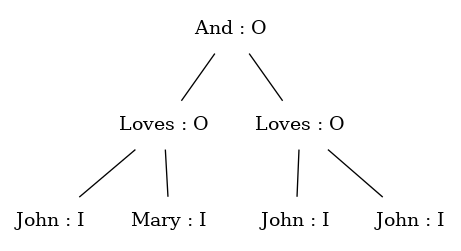
\includegraphics[scale=0.3]{graph_1.png}
\begin{lstlisting}[language=GFcmd, breaklines=true]
> parse -lang=Ger -cat=O "Johannes liebt Maria und Johannes liebt Johannes" | linearize -lang=Eng
John loves Mary and John loves John
\end{lstlisting}
\end{frame}


\end{document}
